Bubbles present in the channels can significantly disrupt the good functioning of the sensor. These perturbations may range from (1) Flow-rate instability if the air bubbles are dilating/contracting \cite{AirBubbles,bruus2011theoretical,Kang2010}. (2) An increase in flow compliance caused by the absorption of pressure changes in the bubbles \cite{AirBubbles,bruus2011theoretical}. (3) An increase in the flow resistance since the bubbles reduce the width of the channel \cite{AirBubbles}. (4) Damages to the cell culture caused by the interfacial tension between the bubble and the liquid which may even result in cell death \cite{AirBubbles,Kang2010}. (5) Aggregation of particles at the interfaces \cite{AirBubbles}. (6) Damage to the wall functionalization of the channel \cite{AirBubbles,Kang2010}. \par

Although they are known to be recalcitrant, some techniques can be used to minimize their impact.  Before dealing with the bubbles, it is important to know their origin in the microfluidics setup and how they form. (1) Some residual bubbles may lodge themselves in the channel after filling it with liquid \cite{bruus2011theoretical,AirBubbles}. (2) Some may be introduced when mixing a second liquid in the channel \cite{AirBubbles}. (3) Some may be induced by porous materials such as PDMS\cite{AirBubbles}. (4) Leaks in the microfluidics setup may introduce bubbles \cite{AirBubbles}. (5) Dissolved gas in the liquid may create them, especially if a surfactant such as soap is mixed with the liquid, or if the liquid is heated, considering that higher temperature presents a lower gas solubility. \cite{AirBubbles,Ufluidix}. \par

Bubbles form themselves from a nucleation point, such as a small irregularity on the surface in which gas can be trapped or regions of low wettability. The nucleation point creates a region of gas phase stability at normal conditions of temperature and pressure \cite{Ufluidix}. When an external pressure is applied, the accumulated gas will either dissolve or expand if the critical radius to form a bubble is reached.  This produces a net growth of the gas in the nucleation point, which may dislodge itself to form a free-moving bubble \cite{Ufluidix,bruus2011theoretical}. The nucleation point will stay in place afterward, generating new bubbles. \par
\begin{figure}[h]
    \centering
    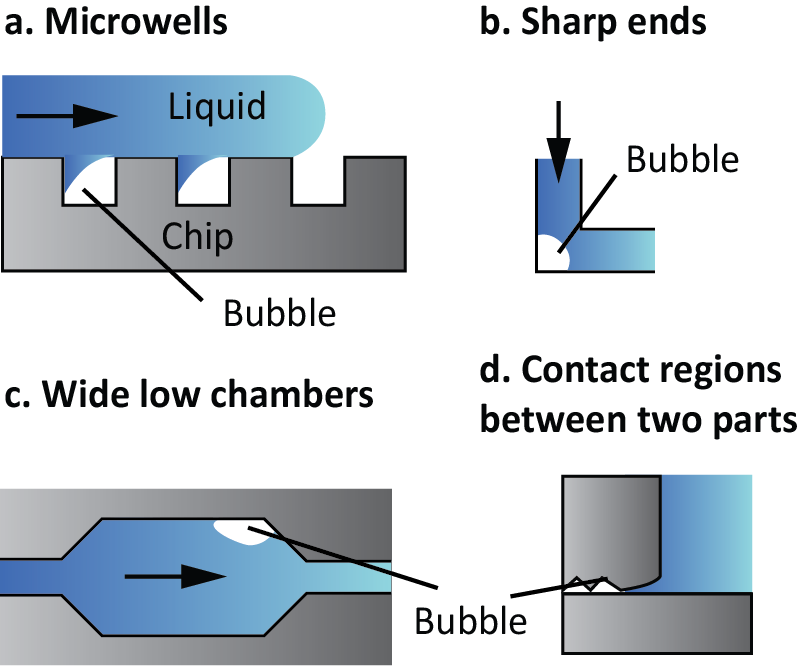
\includegraphics[width=0.7\textwidth]{AirBubble}
    \caption{Origins of air bubbles in a microfluidic channel. \citep{Ufluidix}}
    \label{fig:Airbubble}
\end{figure}
Being aware of their origins, as shown in \autoref{fig:Airbubble}, it is now possible to instigate preventive measures when designing the microfluidic chip to reduce the impacts of the bubbles. (1) Acute angles in the channel should be avoided since bubbles tend to adhere to corners. Dead ends, microwells, and sharp corners should thus be avoided \cite{AirBubbles,Ufluidix}. (2) The channel should be sealed tight using adequate fittings, and contact regions between two separate parts of the device should be bonded adequately, even using Teflon tape or a cladding material such as glues or epoxy if needed \cite{AirBubbles,Ufluidix}. (3) The liquids should be degassed prior to the experiment \cite{AirBubbles}. (4) The surfaces of the channel should be wet to contact angles below 60° to decrease the chance of bubbles getting trapped under sharp angles \cite{Olanrewaju2018,Ufluidix}, and above 30° to prevent corner flow. Corner flow happens when two surface with different wettability composes the walls of a channel. The liquid will flow quicker on some of the wall, resulting in an unequal flow which might create bubbles or even disrupt the channel’s function \cite{Olanrewaju2018}. (5) Pillar-like structures can be added to equalize the speed of the liquid front \cite{Ufluidix}. (6) Wide low chambers or any modification to the width of the channel should be avoided, as liquid tend to circulate at different speed at both sides of the chamber \cite{Ufluidix}. (7) Minimize the number of connectors as they add potential nucleation points for bubbles \cite{Ufluidix}.\par

Despite taking such precautions, bubbles may still remain a problem. In such case, corrective measures should be taken during the experiment. (1) Increasing the pressure inside the channel or sending pressure pulses might be sufficient to dislodge or dissolve the bubbles. Liquid under high pressure present a higher gas solubility \cite{AirBubbles,Ufluidix,bruus2011theoretical}. (2) Applying a higher pressure at both inlet and outlet might be sufficient to dissolve the bubbles into the channel material \cite{AirBubbles,Ufluidix}. (3) Adding degassing systems such as bubble traps or bubble detector to the channel. Some channel geometries have been demonstrated to help trapping or dissolving bubbles. Permeable materials also work to capture bubbles. Finally, hydrophobic materials tend to capture bubbles \cite{AirBubbles,Ufluidix,Olanrewaju2018,bruus2011theoretical,Kang2010}. (4) Flushing the channel with ethanol or a mix of ethanol and water before the experiment can help to remove stuck bubbles, since ethanol has a lower wetting angle than water \cite{Ufluidix}. \par

Bubble traps can be created only by adding cylindrical or hemispherical shapes in the channel path, although hemispherical ones were found to offer superior performances, consistently keeping a higher bubble occupation ratio \cite{Kang2010}. Such traps can be called active or passive depending on if they dissipate the bubbles or merely trap them in the channel. Active bubble traps have the advantage of performance, since the bubbles are taken out of the channel, but they require complex peripheral modules such as vacuum pumps to operate \cite{AirBubbles,Ufluidix,Kang2010}. The passive traps can also dissipate bubbles when an external pressure is applied if they are used in a porous channel substrate such as PDMS. Passive traps only work for hydrophobic surfaces. When used in hydrophilic ones, the bubbles simply slide off the surfaces of the channel when any external pressure is applied \cite{Kang2010}.